% import
\documentclass[conference]{IEEEtran}
\IEEEoverridecommandlockouts
\usepackage{cite}
\usepackage{amsmath,amssymb,amsfonts}
\usepackage{algorithmic}
\usepackage{graphicx}
\usepackage{textcomp}
\usepackage{xcolor}
\usepackage{diagbox}
\usepackage{hyperref}
\usepackage{color, colortbl}
\usepackage{multirow}
\def\BibTeX{
    {\rm B\kern-.05em{
        \sc i\kern-.025em b
    }\kern-.08em T\kern-.1667em\lower.7ex\hbox{E}\kern-.125emX}
}

% url & cite styling
\hypersetup{
    colorlinks=true,
    citecolor=black,
    urlcolor=cyan,
    linkcolor=black
}

% color definition
\definecolor{moreratio}{rgb}{0,1,0}
\definecolor{lessratio}{rgb}{0.95,0.5,0.5}
\definecolor{tableheader}{rgb}{0.8,0.8,0.8}

% renew some commands (to Indonesian Language)
\renewcommand{\abstractname}{Abstrak}
\renewcommand{\IEEEkeywordsname}{Kata Kunci}
\renewcommand{\tablename}{Tabel}
\renewcommand{\figurename}{Gambar}
\renewcommand{\refname}{Referensi}

% document start
\begin{document}

\title{Algoritma Pencarian untuk Pemetaan Kecocokan pada Program Pertukaran Ginjal}

% author
\author{\IEEEauthorblockN{Fazat Nur Azizah}
\IEEEauthorblockA{fazat@informatika.org}
\and
\IEEEauthorblockN{Ardian Umam}
\IEEEauthorblockA{ardian@informatika.org}
\and
\IEEEauthorblockN{Leonardo}
\IEEEauthorblockA{leonardow41@gmail.com}
}

\maketitle

\begin{abstract}
Sebelum transplantasi ginjal dilakukan, pendonor dan pasien calon penerima ginjal harus merupakan pasangan yang cocok.
Faktanya, tidak jarang ketidakcocokan terjadi di antara pasangan donor-resipien, menimbulkan masalah ketersediaan ginjal.
Untuk menyelesaikan masalah ketersediaan ini, Program Pertukaran Ginjal (\textit{Kidney Exchange program}) diciptakan agar
pasangan-pasangan ketidakcocokan dapat melakukan pertukaran ginjal dengan pasangan ketidakcocokan lainnya, membuat pendonoran
silang. Namun karena sangat banyaknya pasangan ketidakcocokan, mencari pemetaan kecocokan dari sekumpulan pasangan ketidakcocokan
bukanlah hal yang mudah. Oleh karena itu, algoritma pencarian pemetaan kecocokan dibuat. Algoritma yang sudah ada, \textit{Edmond's Algorithm},
tidaklah optimal karena sifatnya yang menutup kemungkinan terjadinya pertukaran tiga arah atau lebih. Pada paper ini,
dengan memodifikasi algoritma pencarian pemetaan kecocokan dua arah yang sudah ada, diimplementasikan algoritma pencarian
pemetaan kecocokan \textit{N} arah. Berdasarkan hasil pengujian, menggunakan data berisikan 3000 pasangan ketidakcocokan,
terbukti bahwa algoritma \textit{N} arah adalah algoritma yang superior dibandingkan dengan algoritma dua arah apabila diukur
menggunakan metrik efisensi pencocokan (\textit{matching efficiency}). Peningkatan efisiensi pencocokan yang didapatkan secara
rata-rata mencapai 7.75\% jika dibandingkan dengan efisiensi pencocokan yang didapatkan oleh \textit{Edmond's Algorithm}.
\end{abstract}

\begin{IEEEkeywords}
transplantasi ginjal, pertukaran ginjal, algoritma pencarian pemetaan kecocokan
\end{IEEEkeywords}

\section{Pendahuluan}
Transplantasi ginjal merupakan metode perawatan yang paling direkomendasikan untuk penyakit-penyakit ginjal yang serius\cite{roth2005}.
Setiap tahunnya, di Indonesia sendiri, terdapat lebih dari 100,000 pasien yang memiliki kebutuhan ginjal transplan. Namun
hanya sekitar 20\% dari pasien-pasien tersebut yang bisa mendapatkan transplantasi\cite{wiradarma}. Hal ini terjadi karena
adanya masalah finansial, pandangan masyarakat, dan yang paling umum, masalah ketersediaan.
Meskipun jumlah pendonor setiap tahunnya semakin meningkat\cite{roth2006}, masalah ketersediaan ginjal tetaplah ada
dikarenakan oleh banyaknya kriteria medis yang harus dipenuhi oleh pasangan donor-resipien sebelum operasi dapat dilakukan\cite{wiradarma}.
Pendonor harus memiliki ginjal yang sehat, golongan darah yang cocok dengan resipien, dan tidak memiliki penyakit yang dapat
menular melalui darah. Selain itu, sistem imun dari pasien juga harus dapat menerima ginjal pendonor tanpa membunuh ginjal yang bersangkutan.

\subsection{Transplantasi Ginjal}
\begin{table}[htbp]
    \caption{Kompatibilitas Golongan Darah Penerima dan Pemberi Donor Ginjal \cite{raja}}
    \begin{center}
    \def\arraystretch{1.5}
    \begin{tabular}{|c|c|c|c|c|}
    \hline
    \cellcolor{tableheader}\backslashbox{\textbf{Resipien}}{\textbf{Donor}}&\cellcolor{tableheader}\textbf{O}&\cellcolor{tableheader}\textbf{A}&\cellcolor{tableheader}\textbf{B}&\cellcolor{tableheader}\textbf{AB} \\
    \hline
    \cellcolor{tableheader}\textbf{O}&1&0&0&0 \\
    \hline
    \cellcolor{tableheader}\textbf{A}&1&1&0&0 \\
    \hline
    \cellcolor{tableheader}\textbf{B}&1&0&1&0 \\
    \hline
    \cellcolor{tableheader}\textbf{AB}&1&1&1&1 \\
    \hline
    \end{tabular}
    \label{bloodtypecompatibility}
    \end{center}
\end{table}

Terdapat beberapa buah pengujian yang harus dilalui sebelum transplantasi ginjal dapat dilakukan \cite{adrian}.
Uji golongan darah dilakukan untuk donor dan juga resipien. Seorang pendonor hanya dapat melakukan pendonoran apabila
golongan darah pendonor bersifat cocok dengan golongan darah resipien. Seperti yang dapat dilihat pada Tabel \ref{bloodtypecompatibility},
angka 1 mengindikasikan kecocokan dan angka 0 mengindikasikan ketidakcocokan. Pendonor dengan golongan darah O merupakan
\textit{Universal Donor} karena dapat melakukan donor ke semua golongan darah. Resipien dengan golongan darah AB merupakan
\textit{Universal Recipient} karena dapat menerima donor dari semua golongan darah \cite{charge}.
Uji imunitas dilakukan setelah pasangan donor-resipien melewati uji golongan darah \cite{adrian}. Terdapat dua jenis
pengujian yang dilakukan, yaitu uji silang dan uji \textit{Human Leucocyte Antigen} (HLA). Pada uji silang, darah pendonor
dipertemukan dengan darah resipien untuk melihat terjadinya penggumpalan atau tidak. Penggumpalan terjadi apabila sistem imun
dari resipien menganggap darah dari pendonor merupakan benda asing yang harus dieksterminasi\cite{aprilano}. Uji HLA juga
dilakukan untuk menguji perlawanan dari sistem imun pasien terhadap ginjal pendonor, namun digunakan sel tisu dari pendonor
dan resipien melainkan darah \cite{nguyen}. Setelah semua pengujian selesai, uji serologi dilakukan pada pendonor untuk
menguji apakah terdapat penyakit yang dapat menular melalui darah pada pendonor \cite{aprilano}.

\subsection{Program Pertukaran Ginjal}
Karena banyaknya pasangan donor-resipien yang tidak cocok akibat prasyarat-prasyarat transplantasi, program pertukaran
ginjal bernama \textit{Kidney Paired Donation} (KPD) diciptakan agar pasangan donor-resipien ketidakcocokan dapat mempertukarkan
ginjal dengan pasangan ketidakcocokan lainnya, membuat pendonoran silang menjadi mungkin \cite{raja}. Pertukaran ginjal
antar-pasangan dapat dilakukan secara dua arah, tiga arah, dan dapat dilakukan hingga \textit{N} arah.

\begin{figure}
    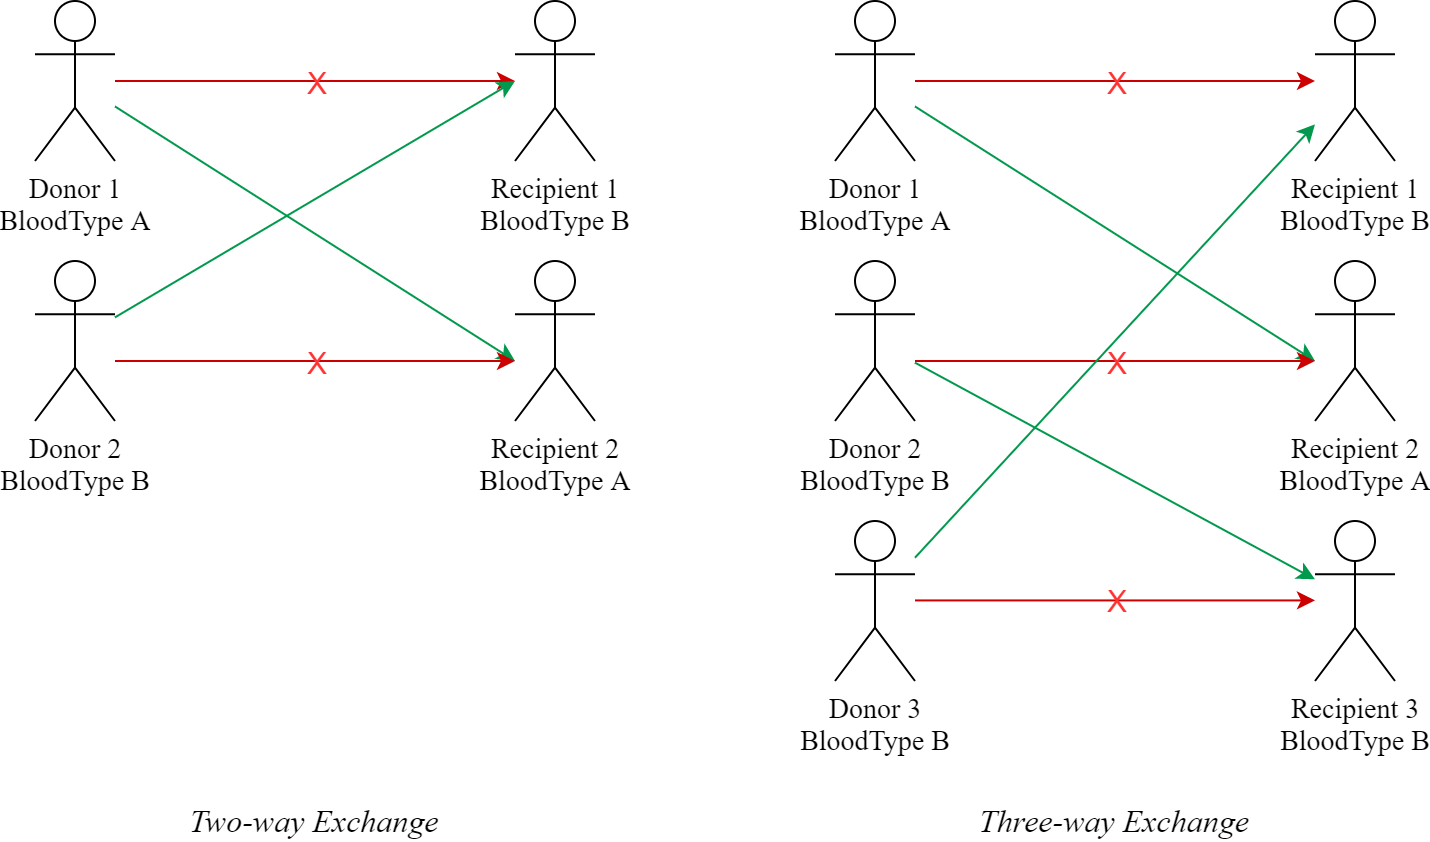
\includegraphics[width=0.5\textwidth]{images/kidney-exchange.png}
    \caption{Pertukaran dua arah(kiri) dan tiga arah(kanan) pada Program Pertukaran Ginjal}
\end{figure}

Karena banyaknya pasangan ketidakcocokan, rumah sakit-rumah sakit tidak dapat secara mudah mendapatkan solusi pencocokan
yang optimal untuk sekumpulan pasangan-pasangna ketidakcocokan. Dibutuhkan algoritma untuk mencarikan pemetaan kecocokan.
Salah satu algoritma yang diketahui untuk menyelesaikan permasalahan ini adalah \textit{Edmond's Algorithm} \cite{raja}.
Pada \textit{Edmond's Algorithm}, kumpulan pasangan ketidakcocokan direpresentasikan dengan suatu graf dengan setiap simpul
yang adalah pasangan ketidakcocokan dan sisi yang merupakan arah pencocokan antar-pasangan yang mungkin. Algoritma ini berfokus
untuk mencarikan kecocokan terlebih dahulu untuk pasangan-pasangan dengan prioritas tinggi sehingga pasien-pasien yang lebih
membutuhkan transplantasi dapat mendapatkan pertukaran terlebih dahulu. Algoritma lain pada lingkup kerja ini adalah algoritma
\textit{First Accept Heuristic Match} \cite{raja} yang menggunakan heuristik dimana pasangan yang registrasi lebih dulu akan
mendapatkan kecocokan terlebih dahulu.

Algoritma-algoritma ini dinamakan algoritma pencarian pemetaan kecocokan. Bagus atau tidaknya algoritma-algoritma ini diukur
menggunakan metrik performa Efisiensi Pencocokan dan Waktu Eksekusi Algoritma \cite{tullis}. Efisiensi pencocokan merepresentasikan
berapa banyaknya pasangan yang mendapatkan kecocokan dari semua pasangan yang ada, ditulis dalam bentuk persentase. Waktu Eksekusi
Algoritma adalah metrik yang mengukur seberapa lama waktu jalannya algoritma dimulai dari \textit{input} masuk hingga \textit{output}
keluar, diukur dalam milisekon (ms). Algoritma pencarian pemetaan kecocokan terbaik merupakan algoritma yang mampu menghasilkan
efisiensi pencocokan yang tinggi dalam waktu eksekusi yang singkat, yang berarti lebih banyak pasien yang lebih dapat terselamatkan
secepat mungkin.

Meskipun \textit{Edmond's Algorithm} dan \textit{First Accept Heuristic Match} sudah ada, algoritma-algoritma
tersebut hanya dapat mengembalikan pertukaran dua arah. Hal ini merupakan suatu batasan karena algoritma-algoritma
ini menutup kemungkinan dicarikannya solusi dengan pertukaran tiga arah atau lebih.

\section{Metodologi}
Berdasarkan masalah-masalah dari algoritma yang sudah dijelaskan pada bab sebelumnya, dibutuhkan algoritma pencarian
pemetaan kecocokan \textit{N} arah untuk kumpulan pasangan ketidakcocokan. Dengan memodifikasi algoritma-algoritma yang
ada, algoritma-algoritma baru dapat dibuat.

\subsection{Modifikasi-modifikasi untuk Algoritma yang sudah ada}
Sebelum algoritma baru dibuat, struktur data dari kumpulan pasangan ketidakcocokan perlu didefinisikan ulang. Graf Kompatibilitas
yang digunakan pada \textit{Edmond's Algorithm} adalah graf tak berarah \cite{raja}, yang berarti sisi pada graf merepresentasikan
kecocokan antara dua simpul, sehingga untuk mencari kecocokan antar pasangan, algoritma hanya perlu mendeteksi sisi pada graf kompatibilitas
yang sudah ada. Hal ini menutup kemungkinan terdeteksinya kecocokan tiga arah atau lebih. Apabila dilakukan modifikasi untuk digunakan
algoritma deteksi siklus dan bukan deteksi sisi untuk menggantikan ini, algoritma-algoritma yang sudah ada akan mampu mendeteksi
kecocokan \textit{N} arah.
Seperti yang dapat dilihat pada Gambar \ref{edgevscycle}, dengan data yang sama, dengan menggantikan algoritma deteksi sisi dengan
deteksi siklus, kecocokan tiga arah dapat terdeteksi sehingga efisiensi pencocokan yang didapat meningkat, membuahkan hasil yang lebih baik.

\begin{figure}[h]
    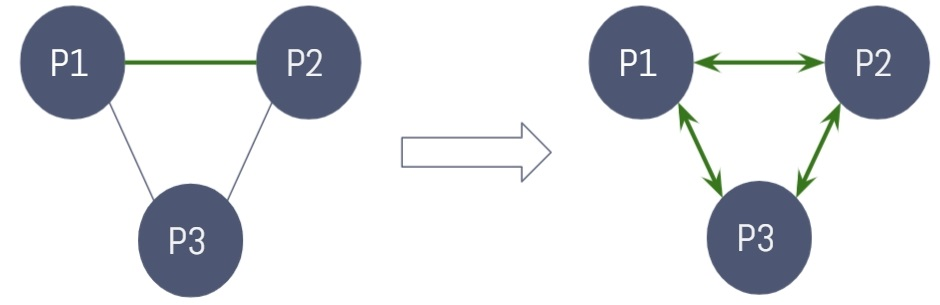
\includegraphics[width=0.5\textwidth]{images/edge-vs-cycle-detection.jpg}
    \caption{Deteksi Sisi(kiri) vs. Deteksi Siklus(kanan) pada Graf Kompatibilitas}
    \label{edgevscycle}
\end{figure}

Meskipun dengan mengubah deteksi sisi menjadi deteksi siklus berpotensi meningkatkan efisiensi pencocokan, hal ini
tentunya tidak cukup. Perlu diperhatikan bahwa siklus-siklus yang didapatkan dari graf adalah siklus bolak-balik.
Apabila graf kompatibilitas yang merupakan graf tak berarah dapat diubah menjadi graf berarah, siklus-siklus satu arah
pada graf juga dapat dideteksi dan dikembalikan, yang secara tidak langsung menambahkan jumlah graf yang dikembalikan,
sehingga berpotensi meningkatkan efisiensi pencocokan seperti yang dapat dilihat pada gambar \ref{undirectedvsdirected}.
Graf tak berarah sendiri adalah struktur data yang terdiri dari sekumpulan simpul dan dihubungi oleh sisi, dimana
setiap sisi memiliki arah yang menunjukkan arah pergerakan yang dapat  dilakukan dari suatu simpul ke simpul-simpul
lainnya \cite{sedgewick}. Algoritma deteksi siklus untuk graf berarah digunakan untuk mencari keberadaan jalur satu
arah dari suatu simpul yang kembali ke simpul mulai pada graf \cite{mehta}.

\begin{figure}[h]
    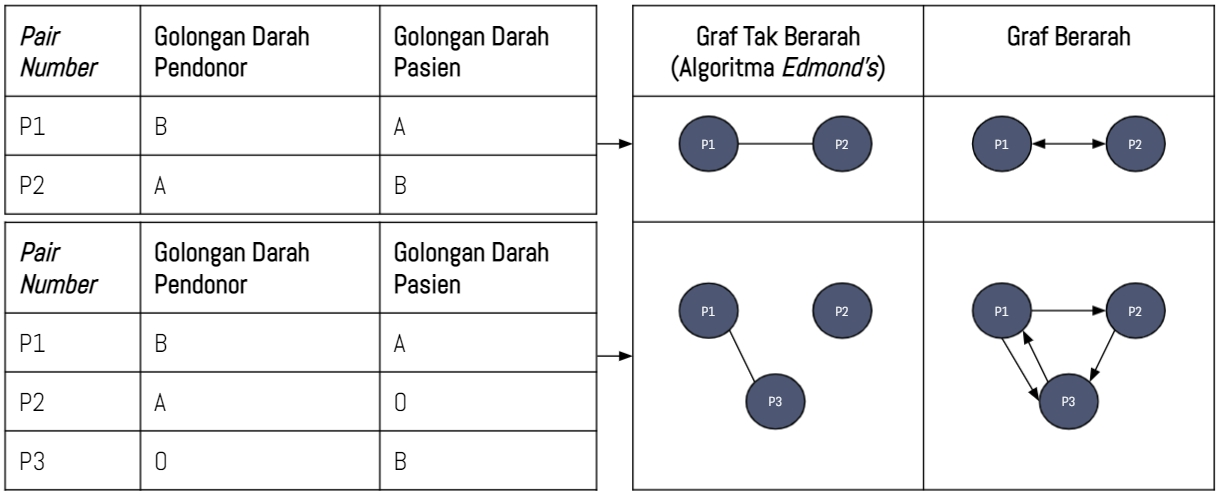
\includegraphics[width=0.5\textwidth]{images/Graf berarah vs Tak Berarah.jpg}
    \caption{Graf Kompatibilitas Tak Berarah vs. Berarah}
    \label{undirectedvsdirected}
\end{figure}

Algoritma deteksi siklus yang digunakan berbeda dengan algoritma deteksi siklus pada umumnya yang mendeteksi apakah
suatu graf memiliki siklus atau tidak (True/False question). Pada implementasi ini, algoritma akan mengumpulkan dan
mengembalikan semua siklus yang dapat terbentuk dari suatu graf kompatibilitas. Setiap siklus pada list siklus yang
dikembalikan adalah pertukaran ginjal yang mungkin terjadi karena bersifat cocok antar-pasangan. Panjang dari siklus
merepresentasikan \textit{N} pada pertukaran \textit{N} arah (cth. siklus sepanjang 3 merepresentasikan pertukaran
tiga arah). Modifikasi ini dilakukan dengan harapan jumlah siklus yang didapatkan akan meningkat niscaya meningkatkan
efisiensi pencocokan, agar lebih banyak pasien yang dapat terselamatkan.

\subsection{Algoritma Pencarian Pemetaan Kecocokan \textit{N} arah}
Dengan kompatibilitas graf yang berarah dan juga algoritma deteksi siklus, algoritma pencarian pemetaan kecocokan \textit{N}
arah dapat dibuat. Algoritma-algoritma \textit{N} arah ini akan menerima list siklus yang dikembalikan dari algoritma
deteksi siklus yang telah dijelaskan sebelumnya. Keluaran dari algoritma ini adalah list siklus yang telah terreduksi
yang dinamakan sebagai pemetaan kecocokan. Reduksi yang terjadi pada algoritma dilakukan karena setiap pasangan pada graf
kompatibilitas ada pada lebih dari satu siklus pada list siklus masukan. Hal ini tentunya tidak mungkin karena setiap
pasangan hanya dapat memberikan dan menerima tepat satu buah ginjal. Reduksi ini dilakukan untuk mengubah hubungan
\textit{many to many} ini menjadi hubungan \textit{one to one}. Reduksi ini pada umumnya menyebabkan beberapa pasangan
ketidakcocokan untuk tidak mendapatkan kecocokan sama sekali. Oleh karena itu, metrik efisiensi pencocokan digunakan
untuk menilai kualitas algoritma dalam menghasilkan jumlah pasangan yang mendapatkan kecocokan sebanyak-banyaknya dari
kumpulan pasangan ketidakcocokan. 

\subsubsection{First Accept Searching Algorithm}
Algoritma \textit{N} arah yang pertama adalah algoritma \textit{First Accept Searching}. Inspirasi dari algoritma ini adalah
algoritma \textit{First Accept Heuristic Match}. Pendekatan yang digunakan disini adalah untuk mengembalikan siklus-siklus
yang ada terlebih dahulu. Algoritma ini memastikan tidak ada pasangan yang mendapatkan kecocokan lebih dari satu kali dengan
menghilangkan siklus-siklus yang mengandung pasangan-pasangan yang telah ada pada siklus-siklus yang telah dikembalikan.

Algoritma ini menggunakan dua buah parameter. Parameter pertama tentunya adalah nilai \textit{N} ini sendiri, karena
algoritma ini adalah algoritma pencarian pemetaan kecocokan \textit{N} arah. Parameter kedua adalah metode penggunaan
nilai \textit{N}. Nilai \textit{N} dapat digunakan sebagai panjang kecocokan maksimum dan sebagai panjang kecocokan eksak.
Jika metode maksimum digunakan, maka siklus-siklus yang dikembalikan dapat memiliki panjang 2 hingga \textit{N}. Sementara
jika metode eksak digunakan, maka siklus-siklus yang dikembalikan hanya adalah siklus-siklus dengan panjang \textit{N} saja.

Meskipun metode maksimum terlihat lebih unggul dibandingkan metode eksak, tidak selalu terjadi demikian. Sebagai contoh, seperti
yang dapat dilihat pada Gambar \ref{maxvsexact}, saat \textit{N} adalah 5, saat metode maksimum digunakan, siklus-siklus bolak-balik
pada graf akan dikembalikan, sehingga pertukaran lima arah pada graf akan dibuang. Saat metode eksak digunakan, karena algoritma
akan mencari siklus-siklus lima arah, algoritma akan mengembalikan pertukaran lima arah pada graf. Pada kasus ini, efisiensi pencocokan
yang lebih tinggi diperoleh saat metode eksak digunakan, bukan metode maksimum.

\begin{figure}[h]
    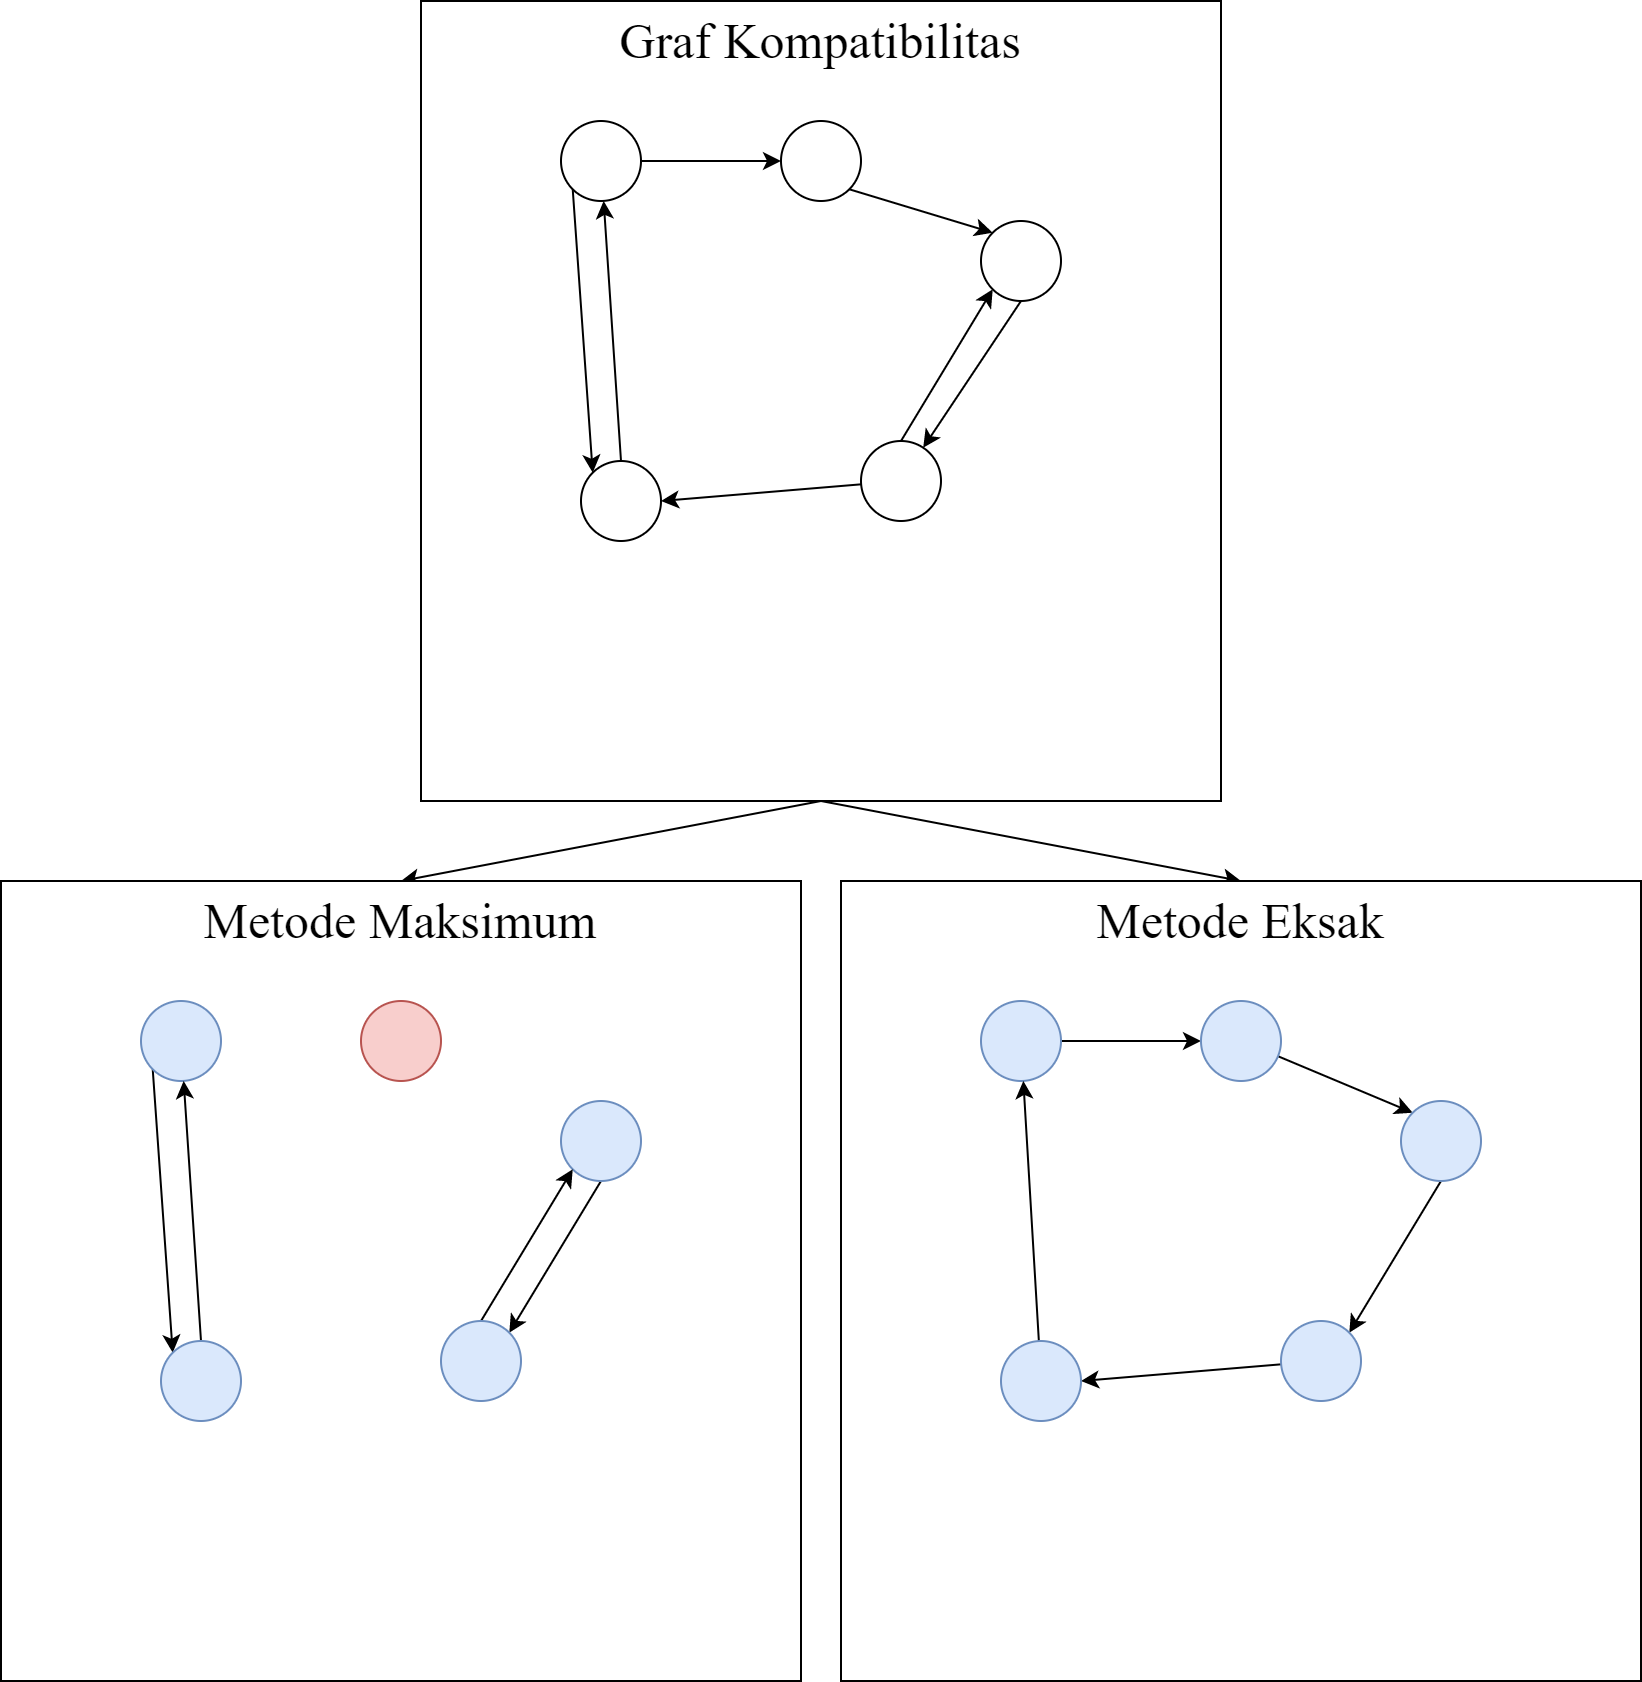
\includegraphics[width=0.5\textwidth]{images/maksimum-vs-eksak.png}
    \caption{Kasus dimana Metode Eksak unggul dibandingkan Metode Maksimum}
    \label{maxvsexact}
\end{figure}

\subsubsection{Priority-based Searching Algorithm}
Algoritma \textit{N} arah yang kedua adalah algoritma \textit{Priority-based Searching}. Insprirasi dari algoritma ini adalah
\textit{Edmond's Algorithm}. Cara kerja dari algoritma ini sangat mirip dengan algoritma \textit{First Accept Searching}, namun
setiap siklus diberikan nilai prioritas sehingga siklus-siklus yang memilii prioritas tinggi dapat dikembalikan terlebih
dahulu dibandingkan yang lainnya. 

Algoritma ini menggunakan tiga parameter. Dua parameter pertama juga digunakan pada algoritma \textit{First Accept Searching},
yaitu nilai \textit{N} dan juga metode penggunaan nilai \textit{N}. Parameter ketiga adalah metode penentuan prioritas. Terdapat
dua metode untuk menentukan prioritas setiap siklus. Metode pertama adalah metode \textit{greedy}. Metode ini memberikan prioritas
yang lebih tinggi pada siklus-siklus yang lebih panjang, dengan harapan dengan banyaknya siklus-siklus panjang yang dikembalikan,
akan meningkatkan efisiensi pencocokan. Metode kedua adalah metode \textit{infrequent}. Metode ini memberikan prioritas tinggi
kepada siklus-siklus dengan pasangan-pasangan yang sulit mendapatkan kecocokan. Pada implementasinya, pasangan-pasangan ini diindikasikan
sebagai suatu simpul yang terhubung oleh jumlah sisi yang sedikit, sehingga pasangan-pasangan tersebut lebih terbatas dari pasangan
lainnya untuk mendapatkan kecocokan dengan pasangan-pasangan ketidakcocokan lainnya.

\section{Experimen dan Analisis}
Sebelum eksperimen dilakukan, \textit{Edmond's Algorithm} diimplementasikan sebagai algoritma \textit{baseline} agar perbandingan
performa antara algoritma \textit{N} arah dan algoritma yang sudah ada dapat dilakukan. Data yang digunakan pada eksperimen ini dapat
ditemukan pada pranala \url{https://rdm.inesctec.pt/dataset/ii-2020-001}. Kode sumber lengkap dari implementasi dan eksperimen dapat
ditemukan pada pranala \url{https://github.com/Mingtaros/Kidney-Exchange-Match-Mapping-System}. Tujuan dari eksperimen dan evaluasi
ini adalah untuk mencari kombinasi algoritma dengan parameter seperti apa kah yang mampu menghasilkan performa terbaik berdasarkan
metrik-metrik yang telah ditentukan. Melalui eksperimen-eksperimen ini, tentunya juga diuji apakah algoritma \textit{N} arah mampu
mengungguli performa dari algoritma \textit{baseline} yang digunakan, \textit{Edmond's Algorithm}. Seperti yang telah dijelaskan,
pengukuran performa algoritma dilakukan dengan metrik efisiensi pencocokan dan juga waktu eksekusi algoritma.

\subsection{Perbandingan Waktu Eksekusi}
\subsubsection{Perbandingan Waktu Eksekusi untuk Kombinasi Algoritma Berbeda}
Pada eksperimen ini, setiap algoritma akan memproses data berisi 3000 pasangan ketidakcocokan yang telah dipecah-pecah menjadi 30
grup yang setiap grupnya dinamakan sebagai suatu \textit{seed}. Setiap \textit{seed} berisikan 100 pasangan ketidakcocokan. Setiap
algoritma akan dijalankan dengan masing-masing data \textit{seed} 50 kali. Seperti yang dapat dilihat pada gambar \ref{exctimealgo},
setiap poin data pada \textit{boxplot} adalah waktu eksekusi rata-rata dari 50 kali eksekusi untuk setiap data \textit{seed}. Untuk
setiap koordinat Y, terdapat 30 titik data yang masing-masing merepresentasikan waktu eksekusi algoritma untuk \textit{seed} yang bersangkutan. 

\begin{figure}[h]
    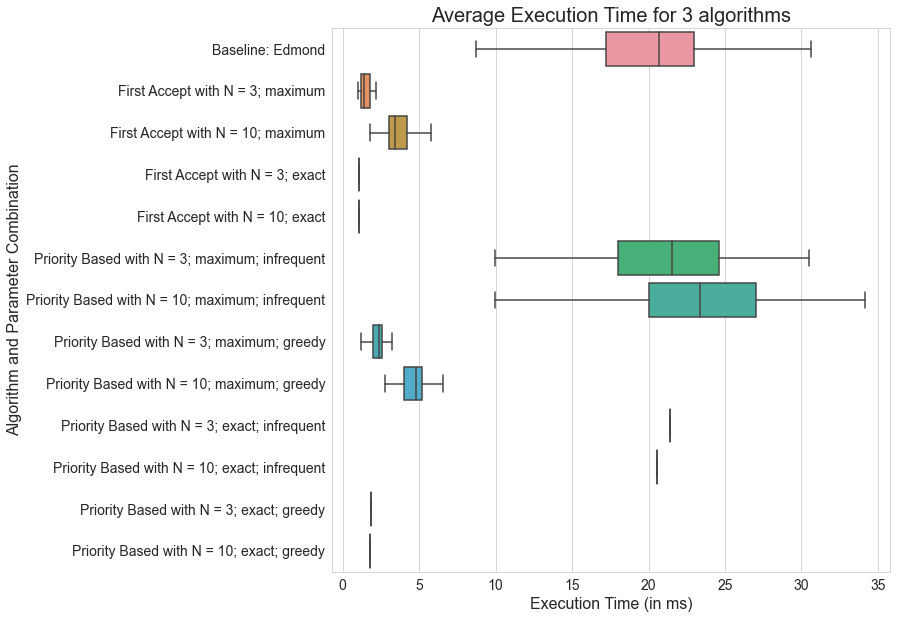
\includegraphics[width=0.5\textwidth]{images/average_execution_time_for_3_algorithms.png}
    \caption{Rata-rata Waktu Eksekusi untuk ketiga Algoritma}
    \label{exctimealgo}
\end{figure}

Seperti yang dapat dilihat pada \textit{boxplot}, \textit{Edmond's Algorithm} dan \textit{Priority-based Searching} dengan
metode penentuan prioritas \textit{infrequent} adalah algoritma-algoritma yang paling lambat. Namun, seperti yang dapat dilihat,
karena tidak ada perbedaan waktu eksekusi yang sangat signifikan antar algoritma, dapat dikonklusikan secara kasar bahwa
perbedaan waktu eksekusi antar algoritma dapat diabaikan.

\subsubsection{Perbedaan Waktu Eksekusi untuk Ukuran Data Berbeda}
Eksperimen ini dilakukan untuk melihat pengaruh dari ukuran data yang berbeda terhadap waktu eksekusi dari algoritma pencarian
pemetaan kecocokan. Untuk eksperimen ini, dicatat rata-rata waktu eksekusi setiap algoritma untuk data sebesar 100, 200,
300, 400, 500, 1000, 2000, dan 3000 pasangan ketidakcocokan. Setiap titik data pada Gambar \ref{exctimedata} menandakan waktu
eksekusi algoritma untuk jumlah data yang masing-masingnya dilakukan sebanyak 10 kali.

\begin{figure}[h]
    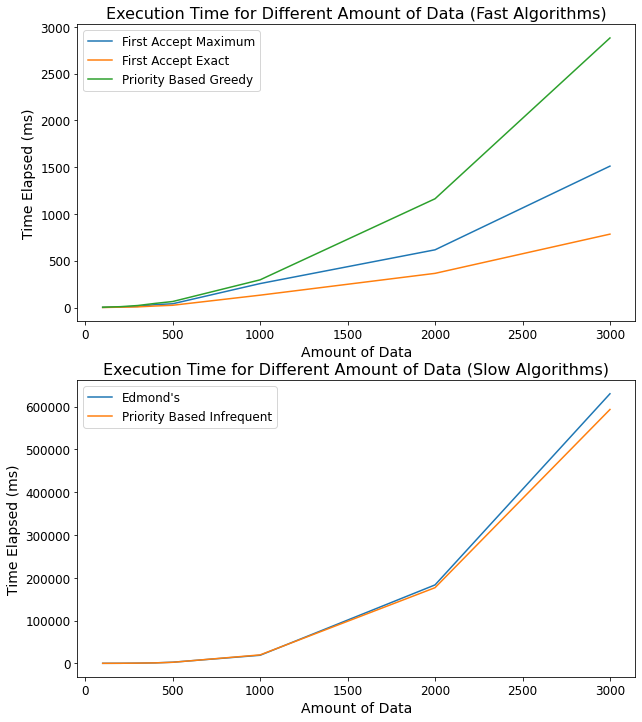
\includegraphics[width=0.5\textwidth]{images/execution_time_for_different_amount_of_data.png}
    \caption{Rata-rata Waktu Eksekusi untuk Ukuran Data Berbeda}
    \label{exctimedata}
\end{figure}

Seperti yang dapat dilihat pada Gambar \ref{exctimedata}, terdapat dua buah diagram yang masing-masing merepresentasikan grup
algoritma yang cepat dan grup algoritma yang lambat. Untuk algoritma yang cepat, saat digunakan 3000 pasangan, waktu maksimum
dari eksekusi algoritma berkisar di 3000 milisekon (30 detik). Sementara untuk algoritma yang lambat, saat digunakan 3000 pasangan,
waktu maksimum dari eksekusi algoritma berkisar di 600000 milisekon (10 menit). Hal ini terjadi karena metode penentuan prioritas
yang mirip pada \textit{Edmond's Algorithm} dan juga metode penentuan prioritas \textit{infrequent} pada algoritma
\textit{Priority-based Searching}. Dari kedua diagram, dapat disimpulkan bahwa relasi antara ukuran data dan waktu eksekusi berbentuk
polinomial dan bukan linear.

\subsection{Perbandingan Efisiensi Pencocokan secara menyeluruh untuk Algoritma Berbeda}
Eksperimen terakhir dilakukan untuk menunjukkan kombinasi algoritma dan parameter mana yang adalah kombinasi terbaik untuk menghasilkan
pemetaan kecocokan dengan efisiensi pencocokan yang tinggi. Pada eksperimen ini, setiap kombinasi diujikan menggunakan 30 data \textit{seed}
berisikan 100 data untuk masing-masing \textit{seed}. Untuk mempermudah pengertian, pada Gambar \ref{matcheffratio}, rasio perkembangan
digunakan untuk menunjukkan besarnya efisiensi pencocokan dari suatu kombinasi algoritma parameter dibandingkan dengan \textit{baseline}
yang merupakan garis lurus horizontal pada gambar. Setiap titik data merepresentasikan rasio efisiensi pencocokan dari algoritma saat
digunakan pada data \textit{seed} tertentu dibandingkan dengan efisiensi pencocokan yang didapatkan oleh \textit{Edmond's Algorithm}.

\begin{figure}[h]
    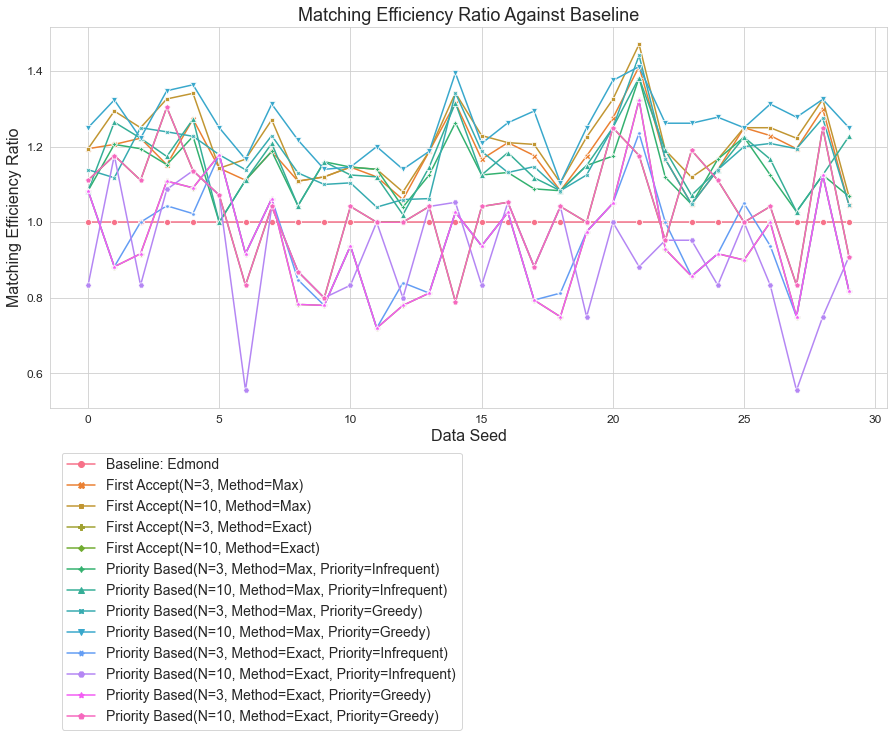
\includegraphics[width=0.5\textwidth]{images/matching_efficiency_ratio_against_baseline.png}
    \caption{Rasio Efisiensi Pencocokan dari Algoritma \textit{N} arah dibandingkan Baseline}
    \label{matcheffratio}
\end{figure}

Untuk menyederhanakan, digunakan tabel \ref{avgmatcheffratio} yang berisikan rata-rata rasio efisiensi pencocokan dibandingkan baseline. Rata-rata yang
digunakan pada tabel adalah rata-rata rasio untuk setiap data \textit{seed}.

\begin{table}[htbp]
    \caption{Average Matching Efficiency Ratio of \textit{N}-way Algorithms compared to Baseline}
    \begin{center}
    \def\arraystretch{1.5}
    \begin{tabular}{|c|c|}
    \hline
    \cellcolor{tableheader}&\cellcolor{tableheader}\textbf{Average} \\
    \cellcolor{tableheader}\textbf{Algorithm}&\cellcolor{tableheader}\textbf{Improvement}\\
    \cellcolor{tableheader}&\cellcolor{tableheader}\textbf{Ratio}\\
    \hline
    Baseline: Edmond's Algorithm&1.0 \\
    \hline
    First Accept(N=3, Method=Max)&\cellcolor{moreratio}1.18 \\
    \hline
    First Accept(N=10, Method=Max)&\cellcolor{moreratio}1.22 \\
    \hline
    First Accept(N=3, Method=Exact)&\cellcolor{lessratio}0.94 \\
    \hline
    First Accept(N=10, Method=Exact)&\cellcolor{moreratio}1.04 \\
    \hline
    Priority Based(N=3, Method=Max, Priority=Greedy)&\cellcolor{moreratio}1.17 \\
    \hline
    Priority Based(N=10, Method=Max, Priority=Greedy)&\cellcolor{moreratio}1.26 \\
    \hline
    Priority Based(N=3, Method=Max, Priority=Infrequent)&\cellcolor{moreratio}1.14 \\
    \hline
    Priority Based(N=10, Method=Max, Priority=Infrequent)&\cellcolor{moreratio}1.16 \\
    \hline
    Priority Based(N=3, Method=Exact, Priority=Greedy)&\cellcolor{lessratio}0.94 \\
    \hline
    Priority Based(N=10, Method=Exact, Priority=Greedy)&\cellcolor{moreratio}1.04 \\
    \hline
    Priority Based(N=3, Method=Exact, Priority=Infrequent)&\cellcolor{lessratio}0.95 \\
    \hline
    Priority Based(N=10, Method=Exact, Priority=Infrequent)&\cellcolor{lessratio}0.91 \\
    \hline
    \end{tabular}
    \label{avgmatcheffratio}
    \end{center}
\end{table}

As can be seen from Table \ref{avgmatcheffratio}, most of \textit{N}-way match map searching algorithm produces higher matching efficiency in
comparison to the baseline, Edmond's Algorithm. However, some algorithms, using the exact method of using \textit{N} parameter,
have worse results compared to baseline. The average matching efficiency of the \textit{N}-way match map searching
algorithms is 7.75\% higher than the baseline algorithm. The higher matching efficiency improvement is obtained when First Accept
Searching algorithm is used when \textit{N} is 10, maximum method of using \textit{N}, with data seed 21, where the improvement
against baseline is 47.06\%.

While \textit{N}-way match map searching algorithms may produce better results, it is worth noting that with \textit{N}-way exchanges
being produced by algorithm may be harder to execute in hospitals since the kidney exchanges have to be operated in the same time. The
implication is that exchanges with lower number of ways are easier to conduct as less hospital resources are needed to conduct the operation.
Therefore, there needs to be an algorithm comparison regarding the average and the maximum exchanges length of the cycles in the match map.
In this experiment, every algorithm and parameter combinations are being tested for 30 data seeds with each containing 100 incompatible pairs. 

\begin{figure}[h]
   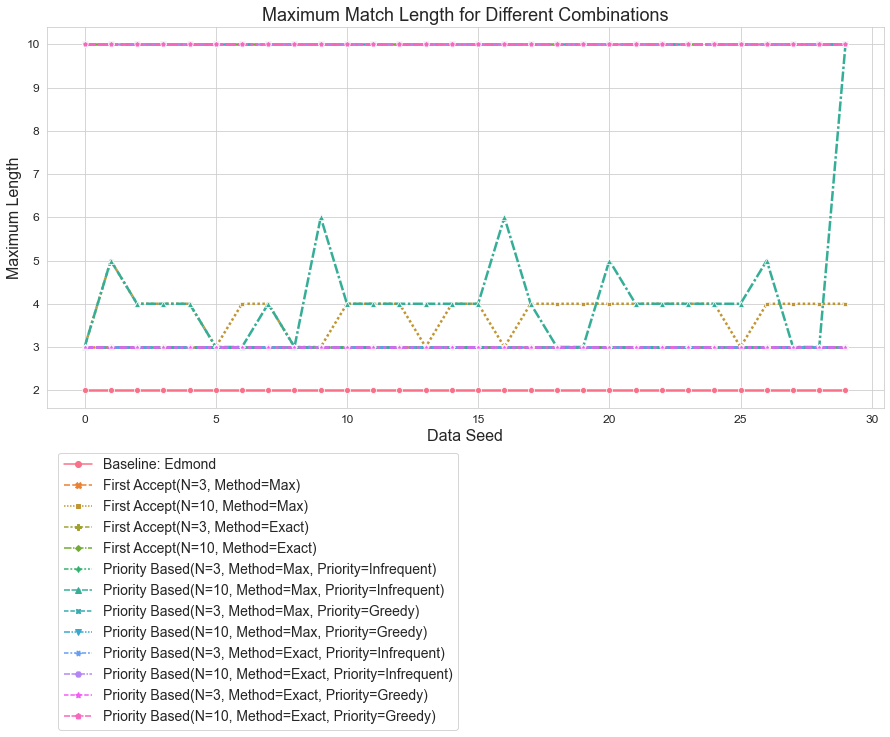
\includegraphics[width=0.5\textwidth]{images/maximum_match_length_for_different_combinations.png}
   \caption{Maximum Match Length for Different Algorithm Combinations}
   \label{figuremaxlength}
\end{figure}

From what can be seen in Figure \ref{figuremaxlength}, Edmond's Algorithm and algorithms with \textit{N} usage method parameter assigned to exact, produced the maximum
length of \textit{N} as the cycles in the produced match map is all of the same length that is \textit{N}.
The more interesting result is that although the parameter \textit{N} is 10, as can be seen with the green and the yellow line, the maximum length is
is not that close to 10. 

\begin{figure}[h]
    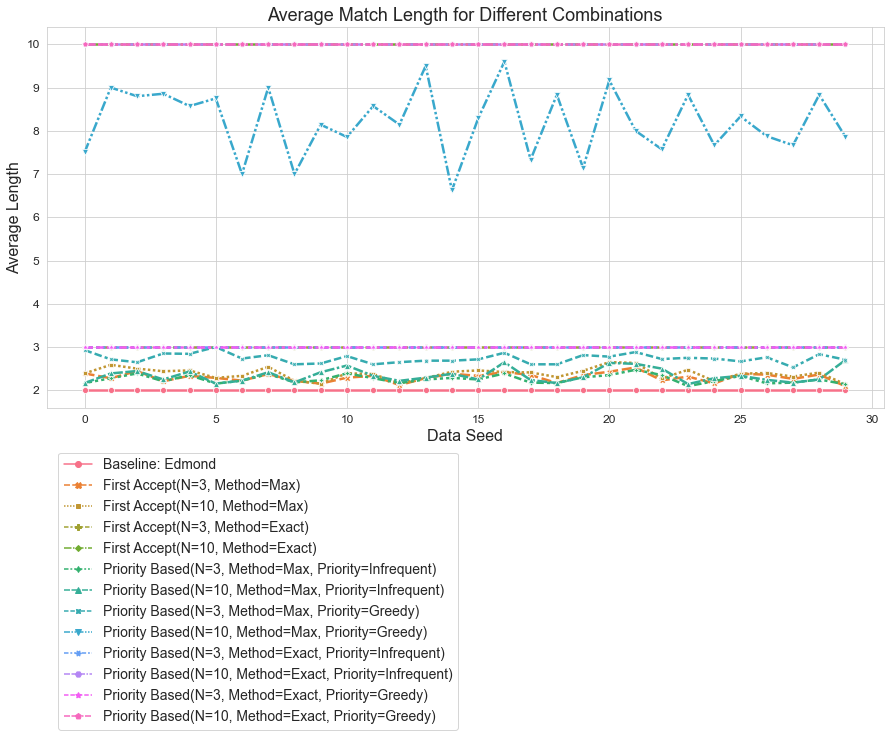
\includegraphics[width=0.5\textwidth]{images/average_match_length_for_different_combinations.png}
    \caption{Average Match Length for Different Algorithm Combinations}
    \label{figureavglength}
\end{figure}

Similar to what can be seen in Figure \ref{figuremaxlength}, in Figure \ref{figureavglength}, Edmond's Algorithm and algorithms with
\textit{N} usage method parameter assigned to exact, produced the average length of \textit{N} as the cycles in the produced match map is all
of the same length that is \textit{N}. Generally, almost every algorithm that uses maximum method of \textit{N} usage produces cycles with the
average length of around 2 to 3, with Priority-based Searching algorithm with N=10, Method=Max, and Priority=Greedy, having an averagely high
average length of exchanges.

\section{Conclusion}
This paper shows that it is a viable option to use \textit{N}-way match map searching algorithms instead of the usual two-way
algorithms such as Edmond's Algorithm for Kidney Paired Donation, with \textit{N}-way algorithms producing better matching efficiency
and competitive execution time in comparison to the baseline, Edmond's Algorithm provided the same dataset. Generally speaking,
the usage of \textit{N}-way algorithms increases matching efficiency by 7.75\%.

With the provided data, First Accept Searching algorithm have a more consistent performance in general compared to Priority-based Searching
algorithm. However, with Priority-based Searching algorithm, the matching efficiency improvement is generally higher with the exception of
when exact method to utilize \textit{N} is being used instead of the maximum method. However, it is worth noting that priority-based searching
algorithm may produce high matching efficiency with the compromise of high average matching length if greedy priority assignment method is being
used. Therefore it can be concluded that First Accept Searching algorithm is the most ideal \textit{N}-way match map searching algorithm to use
in Kidney Exchange Program. 

\section{Related Work}
The idea of the solution, the existing algorithms, and the performance metrics being used as a performance measure are all obtained from
the main reference paper, Web Based Decision Support System for Kidney Exchange by Samy Raja, Prasanna Devi S., and Suryaprakasa Rao K. in
International Journal of Computer Applications \cite{raja}. In that paper, two-way match map searching algorithms are being used to tackle
the problem of the humanely-impossible task of searching the most optimal match map out of an incompatible pairs pool, which becomes the baseline
and the reference of the newer algorithms being implemented in this paper.

\begin{thebibliography}{00}
\bibitem{roth2005} Roth, A. E., Sonmez, T., Unver, M. U. (2005). Kidney Exchange. Quarterly Journal of Economics, 32.
\bibitem{wiradarma} Wiradarma, K. (2016, February 3). Transplantasi Ginjal di Indonesia: Pencapaian dan Hambatannya. Retrieved from klikdokter.com: https://www.klikdokter.com/info-sehat/read/2697086/transplantasi-ginjal-di-indonesia-pencapaian-dan-hambatannya
\bibitem{roth2006} Roth, A. E., Sonmez, T., Unver, M. U., Delmonico, F. L., Saidman, S. L. (2006, September 18). Utilizing List Exchange and Nondirected Donation through ‘Chain’ Paired Kidney Donations. Retrieved from onlinelibrary.wiley.com: https://onlinelibrary.wiley.com/doi/full/10.1111/j.1600-6143.2006.01515.x
\bibitem{adrian} Adrian, K. (2020, May 17). Berbagai Persiapan Donor Ginjal yang Perlu Anda Ketahui. Retrieved from alodokter.com: https://www.alodokter.com/hal-hal-yang-harus-diperhatikan-sebelum-melakukan-donor-ginjal
\bibitem{raja} Raja, S., S., P. D., K., S. R. (2011). Web Based Decision Support System for Kidney. International Journal of Computer Applications (0975 – 8887), 9.
\bibitem{charge} Chargé, S., Hodgkinson, K. (2017, January). Blood: the basics. Retrieved from profedu.blood.ca/: https://profedu.blood.ca/en/transfusion/publications/blood-basics.
\bibitem{aprilano} Aprilano, W. D. (2021, January 20). Teknik Transplantasi Ginjal. Retrieved from alomedika.com: https://www.alomedika.com/tindakan-medis/transplantasi/transplantasi-ginjal/teknik
\bibitem{nguyen} Nguyen, H. D., Williams, R. L., Wong, G., Lim, W. H. (2013, February 13). The Evolution of HLA-Matching in Kidney Transplantation. Retrieved from intechopen.com: https://www.intechopen.com/books/current-issues-and-future-direction-in-kidney-transplantation/the-evolution-of-hla-matching-in-kidney-transplantation
\bibitem{tullis} Tullis, T., Albert, B. (2013, June 3). Performance Metrics. Retrieved from sciencedirect.com: https://www.sciencedirect.com/science/article/pii/B9780124157811000042
\bibitem{sedgewick} Sedgewick, R., Wayne, K. (2020). Directed Graphs. In R. Sedgewick, K. Wayne, Algorithms, 4th Edition (p. 955). New Jersey: Princeton University.
\bibitem{mehta} Mehta, D. (2020, May 27). Detect Cycle in a Directed Graph. Retrieved from geeksforgeeks.org: https://www.geeksforgeeks.org/detect-cycle-in-a-graph/
\end{thebibliography}

\end{document}
